\documentclass[xetex,table,table]{beamer}

\usepackage[autostyle]{csquotes}
\usepackage{hyperref}
\usepackage{color}
\usepackage{xcolor}
\usepackage{setspace}
\usepackage{listings}
\usepackage{minted}
\usepackage{booktabs}
\usepackage{fancyvrb}
\usepackage{fontawesome}
\usepackage{tikz}

\usetheme{metropolis}

\setbeamertemplate{section in toc}[circle]

\usemintedstyle{perldoc}

\newcommand{\myhref}[2]{
  \href{#1}{#2 {\tiny\faExternalLink{}}}
}

\title{License compliance for embedded Linux devices with Buildroot}
\author{Luca Ceresoli --- AIM Sportline\\
  \href{mailto:luca@lucaceresoli.net}{\tt luca@lucaceresoli.net}\\
  \url{https://lucaceresoli.net}
}
\date{\href{https://fosdem.org/2020/schedule/event/buildroot_license_compliance/}{FOSDEM 2020}}

\begin{document}

\maketitle

\begin{frame}{About me}
  \begin{columns}
    \column{0.5\textwidth}
    \includegraphics[width=\textwidth]{../common/images/aim-products.jpg}

    \column{0.5\textwidth}
    \begin{itemize}
    \item Embedded Linux engineer\\
      at AIM Sportline\\
      {\footnotesize\href{https://www.aim-sportline.com/}{www.aim-sportline.com}}
      \begin{itemize}
      \item Develop products on custom hardware
      \item Kernel, drivers, bootloader, FPGA
      \item Integration, build system
      \end{itemize}
    \item Open source enthusiast
      \begin{itemize}
      \item Contributor to the Linux kernel, U-Boot, Buildroot and others
      \end{itemize}
    \end{itemize}
  \end{columns}
\end{frame}

\begin{frame}
  \Huge
  \begin{center}
    {\scalebox{3}{\Huge\faExclamationTriangle}}

    Disclaimer:

    This is not legal advice
  \end{center}
\end{frame}


\section{Buildroot}

\begin{frame}{Build system}
  \begin{center}
    \includegraphics[width=1.0\textwidth]{images/process-1.pdf}
  \end{center}
\end{frame}

\begin{frame}[standout]
  Demo:

  Buildroot basics
\end{frame}


\section{Open-source licensing}

\begin{frame}{Typical license families}
  \begin{columns}

    \column{0.5\textwidth}
      \begin{center}
        {\bf Permissive}\\
        (BSD, MIT, X11\dots)\\
      {\ }\\
      \faCheckCircle\\
      Use, modify, redistribute\\
      {\ }\\
      \faExclamationCircle\\
      Provide license text \\
      {\ }
      \end{center}

    \column{0.5\textwidth}
      \begin{center}
        {\bf Copyleft} \\
        (GPL, LGPL, AGPL\dots)\\
      {\ }\\
      \faCheckCircle\\
      Use, modify, redistribute\\
      {\ }\\
      \faExclamationCircle\\
      Provide license text \\
      Provide source code
      \end{center}

  \end{columns}
\end{frame}

\begin{frame}{Caveats}
  \begin{itemize}
  \item There are many variations
  \item License incompatibility
  \item Info on websites etc might be inaccurate
  \item[\textrightarrow] Check the license {\em in the souce code}
  \end{itemize}
\end{frame}

\begin{frame}{So, what do I have to do?}
  \begin{itemize}
  \item Provide license text
  \item Store source code archives (provide them on request)
    \begin{itemize}
    \item Including the ``scripts used to control compilation and
      installation''
      \begin{itemize}
      \item I.e. the entire buildsystem
      \end{itemize}
    \end{itemize}
  \end{itemize}
\end{frame}


\section{Compliance tools in Buildroot}

\begin{frame}{Compliance tools in Buildroot}
  \begin{center}
    \includegraphics[width=1.0\textwidth]{images/process-full.pdf}
  \end{center}
\end{frame}

\begin{frame}[standout]
  Demo:

  {\tt make legal-info}
\end{frame}


\section[Implementing {\tt legal-info}\\in Buildroot packages]
        {Implementing {\tt legal-info}  in Buildroot packages}

\begin{frame}[fragile]{Add license info to a package}

  {\tt package/vlc/vlc.mk}
  \begin{minted}[frame=single,autogobble,fontsize=\footnotesize]{makefile}
    VLC_LICENSE = GPL-2.0+, LGPL-2.1+
    VLC_LICENSE_FILES = COPYING COPYING.LIB
  \end{minted}

  {\tt package/vlc/vlc.hash}
  \begin{minted}[frame=single,autogobble,fontsize=\footnotesize]{text}
    sha256 8177f975...1b880643  COPYING
    sha256 dc626520...032fe551  COPYING.LIB
  \end{minted}
\end{frame}

\begin{frame}[fragile]{Your own closed source program}

  {\tt package/myapp/myapp.mk}
  \begin{minted}[frame=single,autogobble,fontsize=\footnotesize]{makefile}
    MYAPP_LICENSE = Proprietary
    MYAPP_REDISTRIBUTE = NO
  \end{minted}
\end{frame}

\begin{frame}{Source from unusual locations}
  \begin{itemize}
  \item Source code is not saved when using
    \begin{itemize}
    \item {\tt <PKG>\_OVERRIDE\_SRCDIR}
    \item {\tt <PKG>\_SITE\_METHOD = local}
    \item[\textrightarrow] Avoid them when releasing
    \end{itemize}
  \end{itemize}
\end{frame}

\begin{frame}{\tt ACTUAL\_SOURCES}
  \begin{itemize}
  \item For some special packages:
    \begin{itemize}
    \item {\tt <PKG>\_SOURCE} contains binaries
    \item {\tt <PKG>\_ACTUAL\_SOURCE} points to the tarball with the actual sources
    \item Only used for pre-built external toolchains
    \end{itemize}
  \end{itemize}
\end{frame}


\section{Conclusions}

\begin{frame}{References}
  \begin{itemize}
  \item The Buildroot user manual ({\small\url{https://buildroot.org/docs.html}})
    \begin{itemize}
    \item[\S] \myhref{https://buildroot.org/downloads/manual/manual.html\#legal-info}
                     {12. Legal notice and licensing}
    \item[\S] \myhref{https://buildroot.org/downloads/manual/manual.html\#_infrastructure_for_packages_with_specific_build_systems}
                     {17.5. Infrastructure for packages with specific build systems}
    \end{itemize}
  \item License Compliance in Embedded Linux with the Yocto Project, Paul
    Barker, ELCE 2019
    (\myhref{https://elinux.org/images/2/20/License_Compliance_in_Embedded_Linux_with_the_Yocto_Project.pdf}{slides},
    \myhref{https://youtu.be/9wRn-9KhiEI?list=PLbzoR-pLrL6pamOj4UifcMJf560Ph6mJp}{video})
    \begin{itemize}
    \item Mostly buildsystem-agnostic
    \end{itemize}
  \end{itemize}
\end{frame}

\begin{frame}
  \begin{columns}
    \column{0.4\textwidth}
    \center

    {\Huge Questions?}

    \column{0.6\textwidth}
    \center

    {\Large Thank you for your attention!}

    \vspace{0.15\textheight}

    {\Large Luca Ceresoli}\\
    \href{mailto:luca@lucaceresoli.net}{luca@lucaceresoli.net}\\
    \url{https://lucaceresoli.net}

    \vspace{0.05\textheight}

    \tiny
    \textcopyright{} Copyright 2020, Luca Ceresoli\\
    Slides released under\\
    Creative Commons Attribution - Share Alike 3.0 License \\
    \url{https://creativecommons.org/licenses/by-sa/3.0/} \\
\end{columns}
\end{frame}


\appendix

\section{Extra slides}

\begin{frame}{Typical license families}
  \begin{table}
    \begin{tabular}{lllll}
      \rotatebox{70}{\bf Public domain}
                            & \rotatebox{70}{\bf Permissive}
                                                   & \rotatebox{70}{\bf LGPL}
                                                                             & \rotatebox{70}{\bf GPL} &\\
      \checkmark            & \checkmark           & \checkmark              & \checkmark           & Can use, modify                \\
      \checkmark            & \checkmark           & \checkmark              & \checkmark           & Can redistribute               \\
                            & \faExclamationCircle & \faExclamationCircle    & \faExclamationCircle & Must provide license text      \\
                            &                      & \faExclamationCircle    & \faExclamationCircle & Must provide source code       \\
                            &                      &                         & \faExclamationCircle & Derived work becomes GPL       \\
    \end{tabular}
  \end{table}
\end{frame}

\end{document}
